%----------------------------------------------------------------------------------------
%	CHAPTER 3
%----------------------------------------------------------------------------------------

\chapter{LITERATURE REVIEW}

This section looks at the relevant related work that has been employed previously to resolve satellite Internet delays and takes a look at three past implementations of PEPs. Section 3.1 gives a brief overview of performance enhancing proxies. Section 3.2 provides a brief recap of the satellite links issues and Section 3.2.1 delves into the research conducted to try to resolve these issues with a focus on PEPs. Section 3.3 and its various subsections detail the PEP categorisations. Section 3.4 compares and contrasts three past PEPs with each other and the PEP in this thesis. Section 3.4.1, 3.4.2 and 3.4.3 examine PEPsal, TCPep and FastSAT respectively.

\begin{figure}[h!]
    \centering
    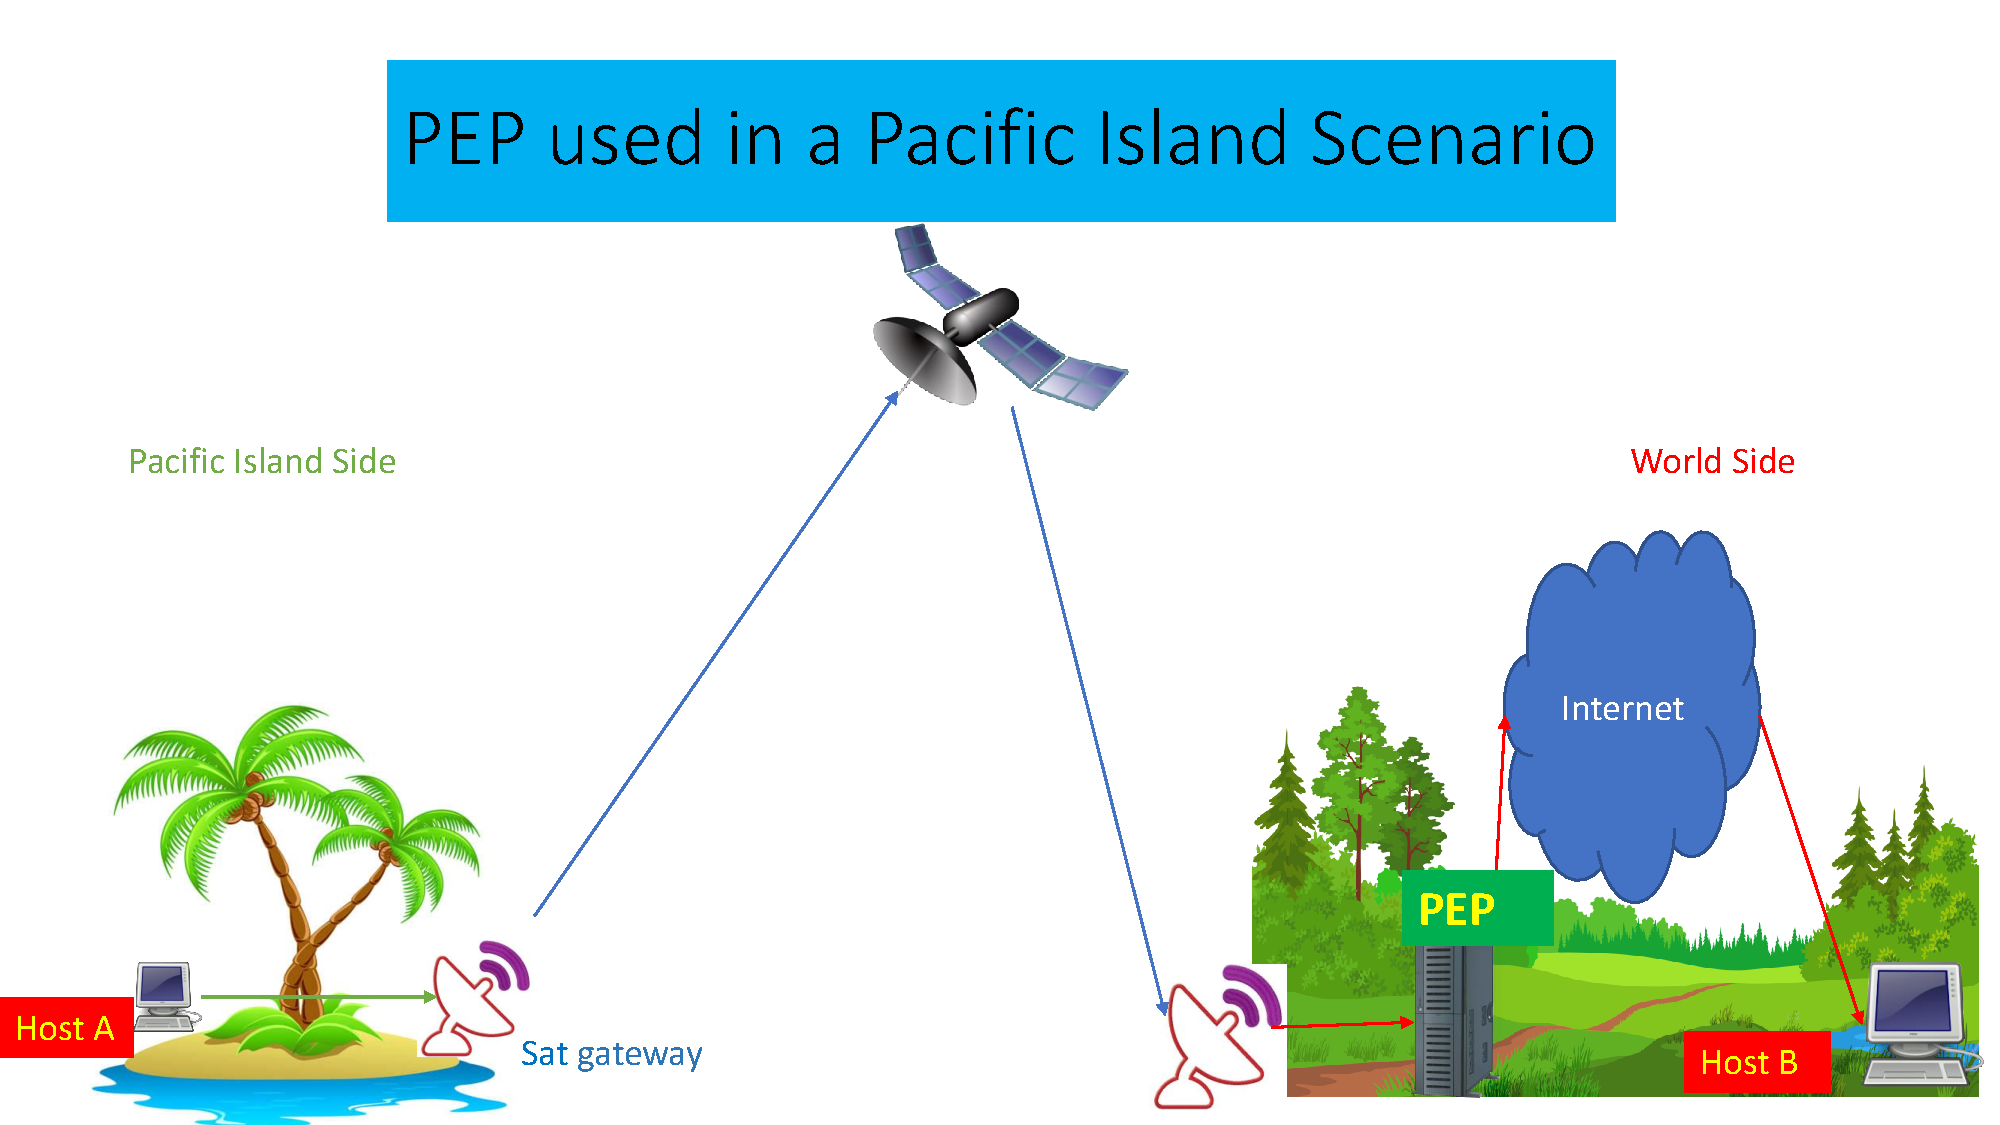
\includegraphics[width=0.95\textwidth]{PEP.pdf}
    \caption{Single PEP on the Island network}
    \label{IslandPEP}
\end{figure}.

\section{Performance Enhancing Proxy}\label{Proxy}
Performance Enhancing Proxies (PEPs) are a technology utilised to prevent the degradation of TCP performance over links with long latencies, such as in the case of TCP over bottleneck satellite links in the Pacific islands ~\cite{6}. (Commercial PEPs are proprietary, so they do not advertise their methods for achieving this). In simple terms, a Performance Enhancing Proxy (PEP) sits between two hosts that are communicating. More precisely, the PEP sits between one host and the degraded link connecting it to the other host ~\cite{6}. In our case, the narrowband bottleneck satellite link is the degraded link connecting our hosts. The PEP is used to effectively give the illusion of shortening the latency between the two hosts and thus mitigating the problems associated with connection latency over a narrowband satellite link. The PEP does this, in most cases, by breaking the connection between the hosts while establishing its own connection with the hosts ~\cite{14}. This type of PEP is called a \emph{connection breaking PEP} and is the most widely and commonly used PEP ~\cite{6}~\cite{14}. Figure \ref{IslandPEP} and \ref{DistributedPEP} give us a visualisation of where the PEP sits in the infrastructure.

\begin{figure}[h!]
    \centering
    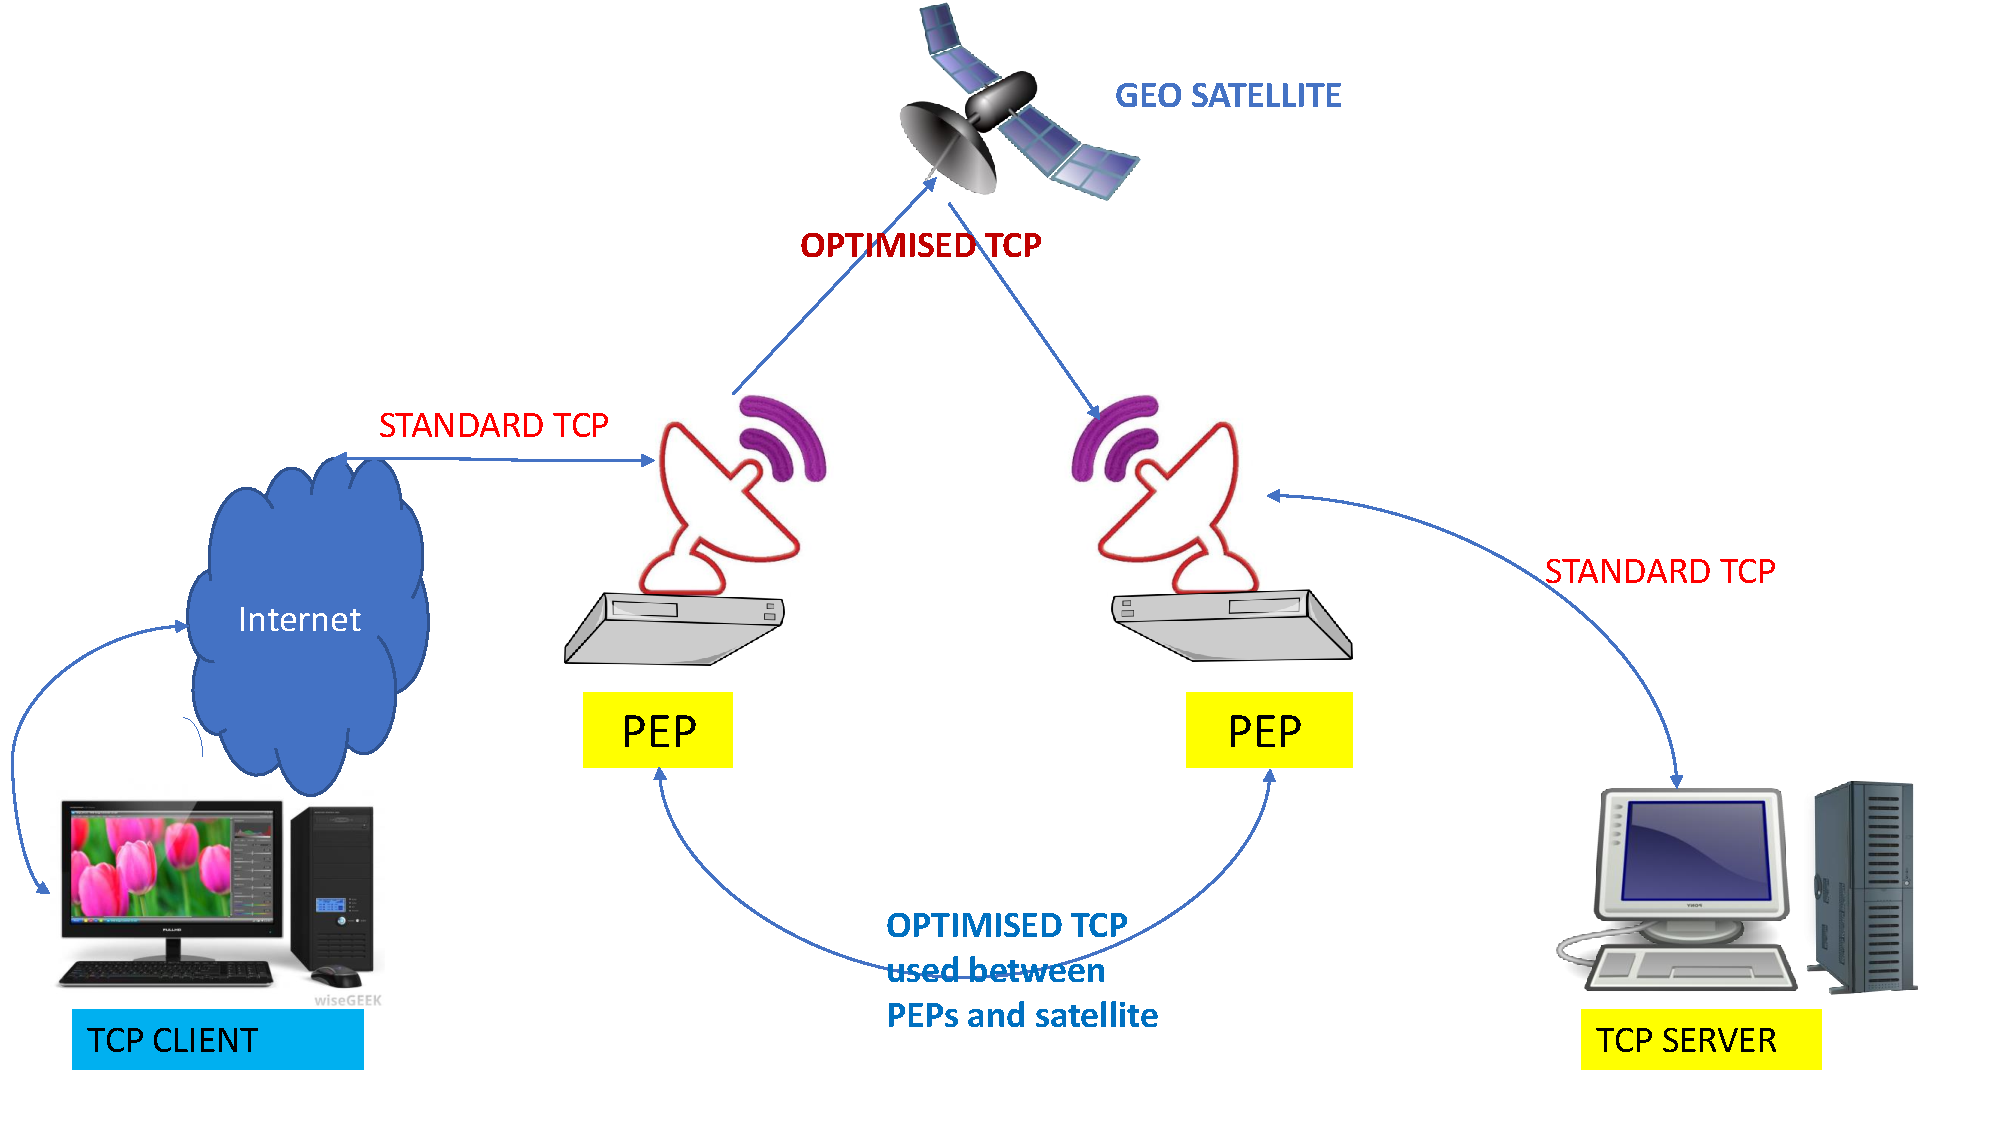
\includegraphics[width=0.9\textwidth]{DistPEPs.pdf}
    \caption{PEP 2nd Diagram}
    \label{DistributedPEP}
\end{figure}

Figure \ref{IslandPEP} shows the PEP sitting between the router of one host endpoint and the satellite link and the other endpoints router and its satellite link. This singular PEP is set up on the world facing side of the satellite link. This is how the PEP in this thesis will be implemented.  \\

Figure \ref{DistributedPEP} shows us a typical visualisation of the TCP client/TCP server connection between client and server. We see satellite connections between client and server is broken up by PEPs in between client and server on both sides of the satellite link. The picture represents the typical set up of a commercial PEP which uses its own proprietary algorithms to optimise the satellite connections ~\cite{6}~\cite{14}. The example here is a TCP client and a ship. Our thesis will focus on the benefits of using the PEP in the Pacific Island environment, but the research is also beneficial for planes and ship satellite communications. \\

\section{History of Satellite Link Issues And Proposed Solutions Including PEPs}\label{History}
Satellite link issues with regards to Internet connectivity, has been fraught with a long history of challenges. The primary culprit behind these challenges is the link latency caused by the long propagation channel between satellites and their terrestrial counterparts in the communication chain. Thus far, this thesis has already detailed the various historical issues/challenges with satellite links. This section will look at the history of proposed solutions resulting from research into these challenges, including PEP variations (Later in this chapter, we will look specifically at past PEP implementations, both open source and commercial). \\

Before we discuss the negatives of satellite links, we should first look at its positives. Satellites can cover extensive geographical areas and can thus provide Internet broadband connectivity to remote areas such as the Pacific Island nations ~\cite{15}. These islands are very difficult to reach via terrestrial infrastructures, with Samoa and Tonga being some of the few islands able to get access to fast broadband connectivity via expensive undersea cables. Most Pacific islands cannot afford this and thus satellite Internet connectivity is the only option at the moment ~\cite{3}~\cite{4}. \\

So while satellites connection are advantageous in some respects, they also have had a long history of challenges in the form of "high delay-bandwidth product, low signal-to-noise ratio, long feedback loop, transmission error, variable Round Trip Time (RTT), and intermittent connectivity" ~\cite{15} which all contribute to extreme queue oscillation. These issues certainly have an adverse effect on the satellite networks quality in terms of Internet connectivity (IP Protocol) ~\cite{15}. \\

Given the length of time satellite latency and the resultant queue oscillation, has been a known problem (over 30 years), one may wonder why there is no clear-cut resolution given over the many years of research. With advancements in technology, it would seem like a solution for our Pacific Island problem would have been found by now ~\cite{21}. \\

The answer has more to do with the socio-economic status of the Pacific Island region in comparison with the rest of the Internet connected world and the general history of satellite Internet. Satellite connections in the 1980s and 90s, or Internet connectivity in general, were not as prevalent in the Pacific as they are now which meant less traffic on the link. Furthermore, Internet data rates, in general, were much slower in the past, not only for the Pacific but most terrestrial network connection. Dial-up speeds were the norm on land in so so the reduced traffic combined with slower rate Internet would have meant we had much less of a bottleneck in the satellite link s of the day to perhaps prompt a need for an urgent fix ~\cite{21}. Even today, in Rarotonga, we only witness queue oscillation when there are over 2000 parallel inbound TCP flows ~\cite{4}. \\

As the Internet became more of a commodity worldwide by the late 1990's, many more millions of users connected to the Internet, so more investment was made into building satellites capable of meeting this demand. The satellites were built with capacities to be able to deal with the size of the terrestrial networks connecting to them and thus effectively removing or significantly reducing any bottleneck effect and eliminating most, if not all, the adverse effects of satellite link latency ~\cite{21}.\\

This leads us back to the present day and the issue of socio-economic status in the Pacific Islands. The number of Internet users on the islands has grown considerably since the 1980s and 90s meaning that they can now generate a significant amount of Internet traffic (parallel TCP sessions) over the link ~\cite{21}. However, unlike their western counterparts such as New Zealand for instance, many of these Pacific Island nations cannot afford the satellite capacity it takes to eliminate a bottleneck link. Hence the need to find a cheap alternative to mitigate the problem for them ~\cite{3}~\cite{4}. 

\subsection{Historical solutions for satellite link issues}

Researchers have proposed many solutions over the years to mitigate the challenges posed by satellite link connections for the Internet ~\cite{7}~\cite{9}. The body of work brought about in trying to resolve these challenges is vast and complex. Instead of trying to summarise the entirety of this enormous body of work in detail, which would consume the remaining space of this thesis, this section will provide surface detail of the type of solutions presented accompanied by references to allow a more comprehensive investigation by the reader if so desired. \\

A recap and summary of the two main problems with satellite links as per the previous chapter:\\

\begin{itemize}

\item Random lossy links unrelated to congestion happen too often to be ignored. Their frequent occurrence and impact on network performance must be taken into account. Error rates have been reported to be as high as 1 in 10-5 which is comparatively much higher than terrestrial routes ~\cite{22}~\cite{25}. TCP regards all losses as due to congestion which triggers the backoff algorithm.

\item The RTT is increased by the large propagation latency to a number that is significantly large enough to cause problems in the network as previously discussed (GEO RTT is typically at 500 ms or slightly above). Excessive queue oscillation and subsequent major packet loss and link underutilisation results from the sender not being able to gauge the state of the link as quickly as it does on terrestrial links ~\cite{7}~\cite{9}.\\

\end{itemize}

Recall that these two factors combine to cause significant problems for the transport layer TCP reliability ~\cite{7}~\cite{9}. TCP \emph{slow start/congestion avoidance} mechanism is severely disrupted resulting in inefficient behaviour typified by unnecessary retransmissions and false timeouts ~\cite{8}~\cite{15}. 

Several research avenues have been explored to solve the abovementioned problem and can be categorised as either improvement to TCP involving only the end hosts ~\cite{10}~\cite{26} or TCP enhancements via the use of PEPs ~\cite{6}~\cite{14}. \\

An option that has been explored is to make TCP more intelligent so that it can distinguish between losses caused by congestion and losses resulting from random datagram errors ~\cite{23}. NASA provided funding for experiments of this nature where \emph{explicit error notification} can be used for satellite links. This would help reduce the backoff algorithm from being triggered prematurely and allow faster opening of the cwnd ~\cite{13}~\cite{23}. So far, results from these studies have not been released publicly or commercially as far as this author is aware. \\

Another TCP extension/improvement was aimed at improving retransmission times but more importantly, enabling TCP to have a better assessment of the available path bandwidth after a period of successive losses via selective acknowledgements (SACKs) ~\cite{24}. Though not explicitly developed for satellite networks, the retransmission efficiency it offers can at least help alleviate one aspect of the satellite link problem.\\

The use of the forward error correction properties of a network code was recently proposed as a solution to the satellite link problem and tested specifically for the Pacific Island region ~\cite{4}~\cite{5}. The network coding was shown to improve TCP performance over a satellite link by hiding packet losses between two TCP hosts on opposite sides of the link ~\cite{4}~\cite{5}.\\

From the TCP improvements proposed via the use of PEPs ~\cite{6}~\cite{14}, the connection breaking/TCP splitting PEPs have been touted as the most effective option by some researchers ~\cite{14}, but they also have their problems. In breaking the fundamental end to end semantics of TCP, they can cause many adverse side effects ~\cite{6}. The TCP PEPs can also be categorised as either integrated or distributed, open source or commercial. This section will only discuss these categorisations briefly, but they will be covered in more depth in Section 3.3 \emph{Pep Catergorisations}.\\

An integrated PEP sits on only one side of the satellite link which is the side representing the last hop for Internet access. These PEPs use TCP or an optimised version of TCP over the satellite leg of their link path and usually require no software or hardware modification to the receiver end ~\cite{6}~\cite{14}. A distributed PEP sits on both sides of the sat link and can, therefore, use a custom transport protocol other than TCP across the satellite link itself. Most commercial PEPs use or permit a distributed architecture ~\cite{6}~\cite{14}. \\

The PEP in this thesis will be open source and using an integrated architecture with TCP for testing and experimentation (although it can also be modified to be used in a distributed architecture too) but will be non-connection breaking. For this reason, this thesis will not be focused on TCP splitting options ~\cite{14}~\cite{27}~\cite{28}. This research will also not focus on commercial implementations of PEPs ~\cite{29} as the source code is proprietary and will also disregard open source distributed PEPs, that use their own specialised transport protocols such as SCPS ~\cite{11}. \\

The PEP in this thesis also uses TCP whereas a past PEP implementation called PEPsal, for instance, uses an enhanced form of TCP called TCP Hybla which has been optimised for better performance to suit satellite links ~\cite{14}. This thesis will only focus on the performance of the PEP itself using standard TCP variants. This PEP is also tested and run on Linux, similarly to PEPsal, PEP solutions not available for Linux will not be considered here. ~\cite{30}~\cite{31}~\cite{32}. \\

The open source non-connection breaking PEP in this thesis is the first of its kind implemented in Linux as far as this author is aware. The next section (3.3) will explain the prior mentioned PEP categorisations in more detail. Then the following section will compare and contrast previously implemented PEPs, such as the previously mentioned PEPsal, with our non-connection breaking PEP. \\

\section{PEP Categorisations}
As part of the literature review on PEPs, it is important to know the PEP categorisations currently in existence. This knowledge helps the reader understand how my PEP is categorised and also how it differs from other PEPs. Generally, the use of PEPs is not recommended unless in an environment where there are no other viable options to improve link performance ~\cite{6}. The consensus is that the fundamental end to end principle of the Internet should always be adhered to where possible and most PEPs break end to end connectivity ~\cite{6}. As mentioned in the introduction, the PEP in our thesis partially addresses this issue as it is an experimental non-connection breaking PEP. Therefore our first categorisation will be for connection breaking PEPs as this has high importance to this thesis. 

\subsection{Connection breaking PEP}
A connection breaking PEP is also referred to as a \emph{TCP splitting PEP} in many manuals. As described in RFC3515, a split connection TCP implementation mimics the endpoint or target host/server of the connection/packet in both directions, thus literally splitting the connection in half (TCP splitting). In an integrated TCP splitting PEP "the PEP... terminates the connection from one end system and originates a separate connection to the other end system" ~\cite{6}. The PEP is managing two separate connections simultaneously so that the endpoints operate as if they are communicating directly with each other. \\

Simply put, the communicating hosts believe there is no middleman. (see Transparency Type below). For example, the intercepting PEP receives a data packet and sends acknowledgements back to the sender to say it has received the packet. The PEP also suppresses the real ACKs coming back from the receiver of sent packets on either side of the split connection. The PEP then forwards the payload data from the packet to the intended target and vice versa ~\cite{6}~\cite{14}. It is essential to keep in mind the connection-breaking concept as the novelty of the PEP in our thesis is the fact it is a non-connection breaking PEP. It is also the first open source non-connection breaking PEP. In Section 4.3.1 "Non-Connection Breaking PEP", this thesis will provide more detail on the reasons for having this as our novelty. These details include the problems inherent in breaking the Internet's fundamental rule of end to end connectivity and the methods utilised by our PEP to partially mitigate these issues. \\

\subsection{PEP distribution type}
There are two types of PEP distribution types:\\
\begin{itemize}
\item Integrated 
\item Distributed\\
\end{itemize}
An Integrated PEP is a single PEP component that connects between a host and the degraded link. The PEP is one node in the connection between the TCP hosts and the degraded link between them. The performance of the link is enhanced at that singular point where the PEP sits. The advantage of having an integrated PEP is that it is a single box and it is neither hardware, software or operating system specific. It is also inexpensive to run and easily maintained or upgraded because it is merely some code sitting on a computer that interacts with the switches/routers ~\cite{6}~\cite{14}. The disadvantage for integrated PEPs is that they only allow standard or advanced TCP protocols on the satellite which means they would have to exclude all proprietary solutions. Even the use of advanced TCP protocols (TCP Hybla etc.) designed for improved performance on a satellite link is somewhat limited as the receiving hosts have to be compatible with this enhanced TCP variant to reap the benefits. Figure \ref{IslandPEP} is an example of an integrated PEP architecture.\\

Distributed PEPs sit on both sides of the problematic link and even on the satellite itself. You could also have a chain of several PEPs along the communication link. This setup is typical with commercial PEPs who use their own proprietary protocols and algorithms, sometimes instead of TCP, to communicate between their proxies. As stated in the PEPsal article, by surrounding and "isolating the satellite link between two PEP agents...it is possible to adopt a proper transport protocol on the satellite link, such as SCPS" ~\cite{14}. SCPS stands for \emph{Space Communications Protocol Specifications}, a non-TCP protocol designed specifically for satellite link traversal ~\cite{11}. Similar proprietary protocols can be applied to this distribution architecture. Figure \ref{DistributedPEP} is an example of a distributed PEP architecture.\\

The PEP in this thesis can be operated both as an integrated type and a distributed type of PEP. 
 
\subsection{PEP layering type}
There are two types here: \\
\begin{itemize}
\item Transport Layer PEPs
\item Application Layer PEPs\\
\end{itemize}

According to RFC 3135 "transport layer PEPs operate at the transport level...they do not modify the application protocol(e.g. HTTP) in any way, but let the application protocol operate end-to-end.  Most transport layer PEP implementations interact with TCP" ~\cite{6}. This is what is known as a TCP PEP and interacts with the TCP Protocol. In environments where we have bursty traffic or prolonged bandwidth delay (as in the case with satellite links) this type of proxy modifies/alters/enhances the TCP behaviour. It can increase ACK spacing to counter bursty traffic that leads to inefficient use of the bandwidth. Alternatively, it can generate local ACK responses to improve the throughput of the link (See previous "Connection Breaking PEP" section for more detail).\\

Application Layer PEPs operate at the application layer (above the transport layer). These types of PEPs are widely used today like Microsoft Proxy Server; the Web Proxy Service is an application layer proxy for the Hypertext Transfer Protocol (HTTP), relay Mail Transfer Agents (MTA) and cache proxies that are used to optimise performance and service availability ~\cite{6}. Application Layer PEPs will not be helpful for dealing with the narrowband satellite link problem in our thesis as it has no bearing on the satellite link issues. PEPsal and TCPep are also \emph{transport layer PEPs}. This thesis will focus only on Transport Layer PEPS.

\subsection{PEP symmetry type}
As defined in RFC3135, a PEPs symmetry type can be either:

\begin{itemize}
\item Symmetric
\item Asymmetric
\end{itemize}

Symmetric PEPs treat both sides of the connection exactly the same, so that the PEPs optimisation is propagated in both directions. Assymetric PEPs treat both sides of the connection differently so that only one link direction performance may be optimised ~\cite{6}. As in the case of the PEP in this thesis, for example, which takes into account one of its sides is facing the satellite link and the other side is facing the island side ~\cite{4}~\cite{5}.  The island senders are on the same side of the satellite connection as the PEP (usually the world side in satellite connections to small islands, ships etc. because this is where most of the data volume comes from) which ensures the quickest ACK returns for the sender's data packets ~\cite{4}. Thus our PEP is assymetric as the link optimisation occurs in the direction facing the island side. See Figure \ref{IslandPEP}.  \\

\subsection{PEP transparency type}
Transparency here is defined as whether the end systems, endpoints, applications or users are aware of the PEP or does the PEP operate entirely transparently/invisible to them. If a PEP requires modifications to be made to any of the end systems, endpoints or applications, then it is considered non-transparent ~\cite{6}. The PEP in our thesis is transparent.

RFC3515 categorises the degree of transparency a PEP can have:\\
\begin{itemize}
\item transparency with respect to the end systems (network-layer transparent PEP) ~\cite{6}.
\item transparency with respect to the transport endpoints (transport-layer transparent PEP) ~\cite{6}.
\item transparency with respect to the applications (application-layer transparent PEP) ~\cite{6}.
\item transparency with respect to the users ~\cite{6}.\\
\end{itemize}

        
\section{Past Implementations Of PEPs}

In this thesis, we show our version of a PEP that uses a non-connection breaking PEP to mitigate the problems with satellite link latency. Before we do this, however, this section examines other PEPs that have been developed and implemented in the past and then finally shows how our version differs.\\
 
List of PEPs considered in this section:
 \begin{itemize}
 \item PEPsal
 \item TCPep
 \item Commercial PEPs
 \end{itemize}
There are many more, but we will restrict ourselves here to the treatment of the two open source PEPS above and a general overview of commercial PEPs which often do not have much detail available for the public. The reader may want to refer to section 2.2.5 "Other Concepts Used In This Thesis" for further information on this topic.

\subsection{PEPsal}
PEPsal was initially developed as part of a research project for experimentation in a university but has since been successfully adopted by a US satellite provider used by the USA and Latin America. It has the advantage of incorporating free software running on Linux ~\cite{14}.

\subsubsection*{TCP splitting}
PEPsal is a connection breaking/TCP splitting PEP first and foremost. It is also considered "the first open source TCP splitting solution created for the GNU/Linux" environment. PEPsal is a simple open source Linux software developed at the University of Bologna, Italy. PEPsal breaks the fundamental rule of internet end to end connection because it is TCP splitting ~\cite{14}. Note that this is one main distinction between PEPsal and the PEP developed in this thesis. \\

One example of a negative consequence of breaking the end to end semantics of a connection with PEPsal is that IPsec cannot be applied end to end with said connection. The two cannot be used together, so this compromises security on the connection. This leaves a network administrator weighing up a choice between the improved link throughput benefits of PEPsal versus the network layer security benefits offered by IPsec ~\cite{14}.

PEPsal intercepts the TCP SYN packet that is coming from the client using netfilter and answers on behalf of the server, and builds up a new connection to the target host using a userspace application that copies data between the two sockets ~\cite{14}.\\

\subsubsection*{PEPsal layering type}
PEPsal is described as a multi layer proxy. It deals with TCP flows in order for it to act as a TCP splitting proxy. This means it operates at the transport layer but also needs access to the IP in order to be able to spoof/pretend to be the other side of a split TCP connection. The PEP in this thesis will also be a multilayer proxy type ~\cite{14}.\\

\subsubsection*{PEPsal distribution type}
PEPsal distribution type can be used as an \emph{integrated PEP} as it can operates out of one singular Linux box (see Figure \ref{IslandPEP}). It can also be used as a \emph{distributed PEP} (See Figure \ref{DistributedPEP}) and have two or more PEPs running on either side of a degraded satellite link to isolate the satellite link from the rest of the network although it still uses TCP only. Pepsal runs its own optimised version of TCP (TCP-Hybla) over the links in both integrated and distributed mode. Other distributed PEPs can run non-TCP protocols as previously mentioned. Like PEPsal, the PEP in this thesis will also be the integrated and distributed type and will remain TCP based ~\cite{14}. \\

\subsubsection*{PEPsal symmetry Type}
PEPsal is classified as both an \textbf{Asymmetric} and \textbf{Symmetric} PEP. If PEPsal is used between a terrestrial host and the gateway to the satellite link, it uses two different operations in either direction: regular TCP on earthbound TCP flows and TCP-Hybla on satellite bound TCP flows, which would be considered asymmetric [26]. The network layer can be configured, however, via modifications on the receiver side, which allow for the same operation on the return trip (Symmetric) ~\cite{6}~\cite{14}.\\

{TCP-Hybla} is an optimised form of TCP developed for PEPsal to negate the link degradation caused by long RTT (Round trip times) in satellite links.  Other Linux TCP variants, however, can also be used with PEPsal, allowing for greater portability across network systems across the board. TCP-Hybla allows faster re-opening of the congestion window (cwnd) ~\cite{26}. TCP Hybla is in Section 2.2.5 if the reader may want to know more about the algorithms workings. The PEP in this thesis will also be both symmetric and asymmetric depending on the network layer configuration.\\

\subsubsection*{PEPsal Summary}
PEPsal is a current solution to the satellite links aforementioned TCP degradation problems caused by long RTT which we address in this thesis. It has many advantages as mentioned earlier, including ease of maintenance or upgrades if required on host servers or the affected satellites ~\cite{6}~\cite{14}.

Ultimately, PEPsal achieves what it was intended for which is to create a viable and cheap/free alternative to commercial "black-box" PEPs. This is also the aim of our proposed PEP. Our proposed PEP differs in that it maintains the end to end connection rule of the Internet as it aims to improve TCP performance over the degraded link while maintaining end to end reliability over the network. As stated in RFC3135, breaking the end to end semantics of a connection has negative implications which for example include, but are not limited to, loss of end to end reliability and disablement of IPsec ~\cite{6}~\cite{14}. 

\subsection{TCPep}
TCPep was created with a slightly different purpose than PEPsal. Like PEPsal and all PEPs in general, it also has the goal of resolving the problems of link degradation. However, it differs from PEPsal and the solution our thesis proposes in a few ways, starting with its primary motivation. \\

Our PEP (and PEPsal) were built to mitigate the link degradation caused by long RTT bandwidth delays caused by bottleneck satellite links. TCPep was created as part of a Dublin University research project, to counter random losses over lossy links (Wireless LAN links). The project owner describes TCPeP as a Performance-Enhancing proxy for TCP over lossy links, combined with Network Coding ~\cite{33}.\\

Most, if not all, TCP congestion control algorithms were created under the assumption that lost packets are caused by congestion. Standard TCP congestion avoidance mechanisms react to the loss of ACKs as a sign of congestion on the network ~\cite{13} Standard TCP congestion control, however, is not designed to compensate for lossy links with high uncorrected error rates ~\cite{13}~\cite{33}.

\begin{figure}[h!]
    \centering
    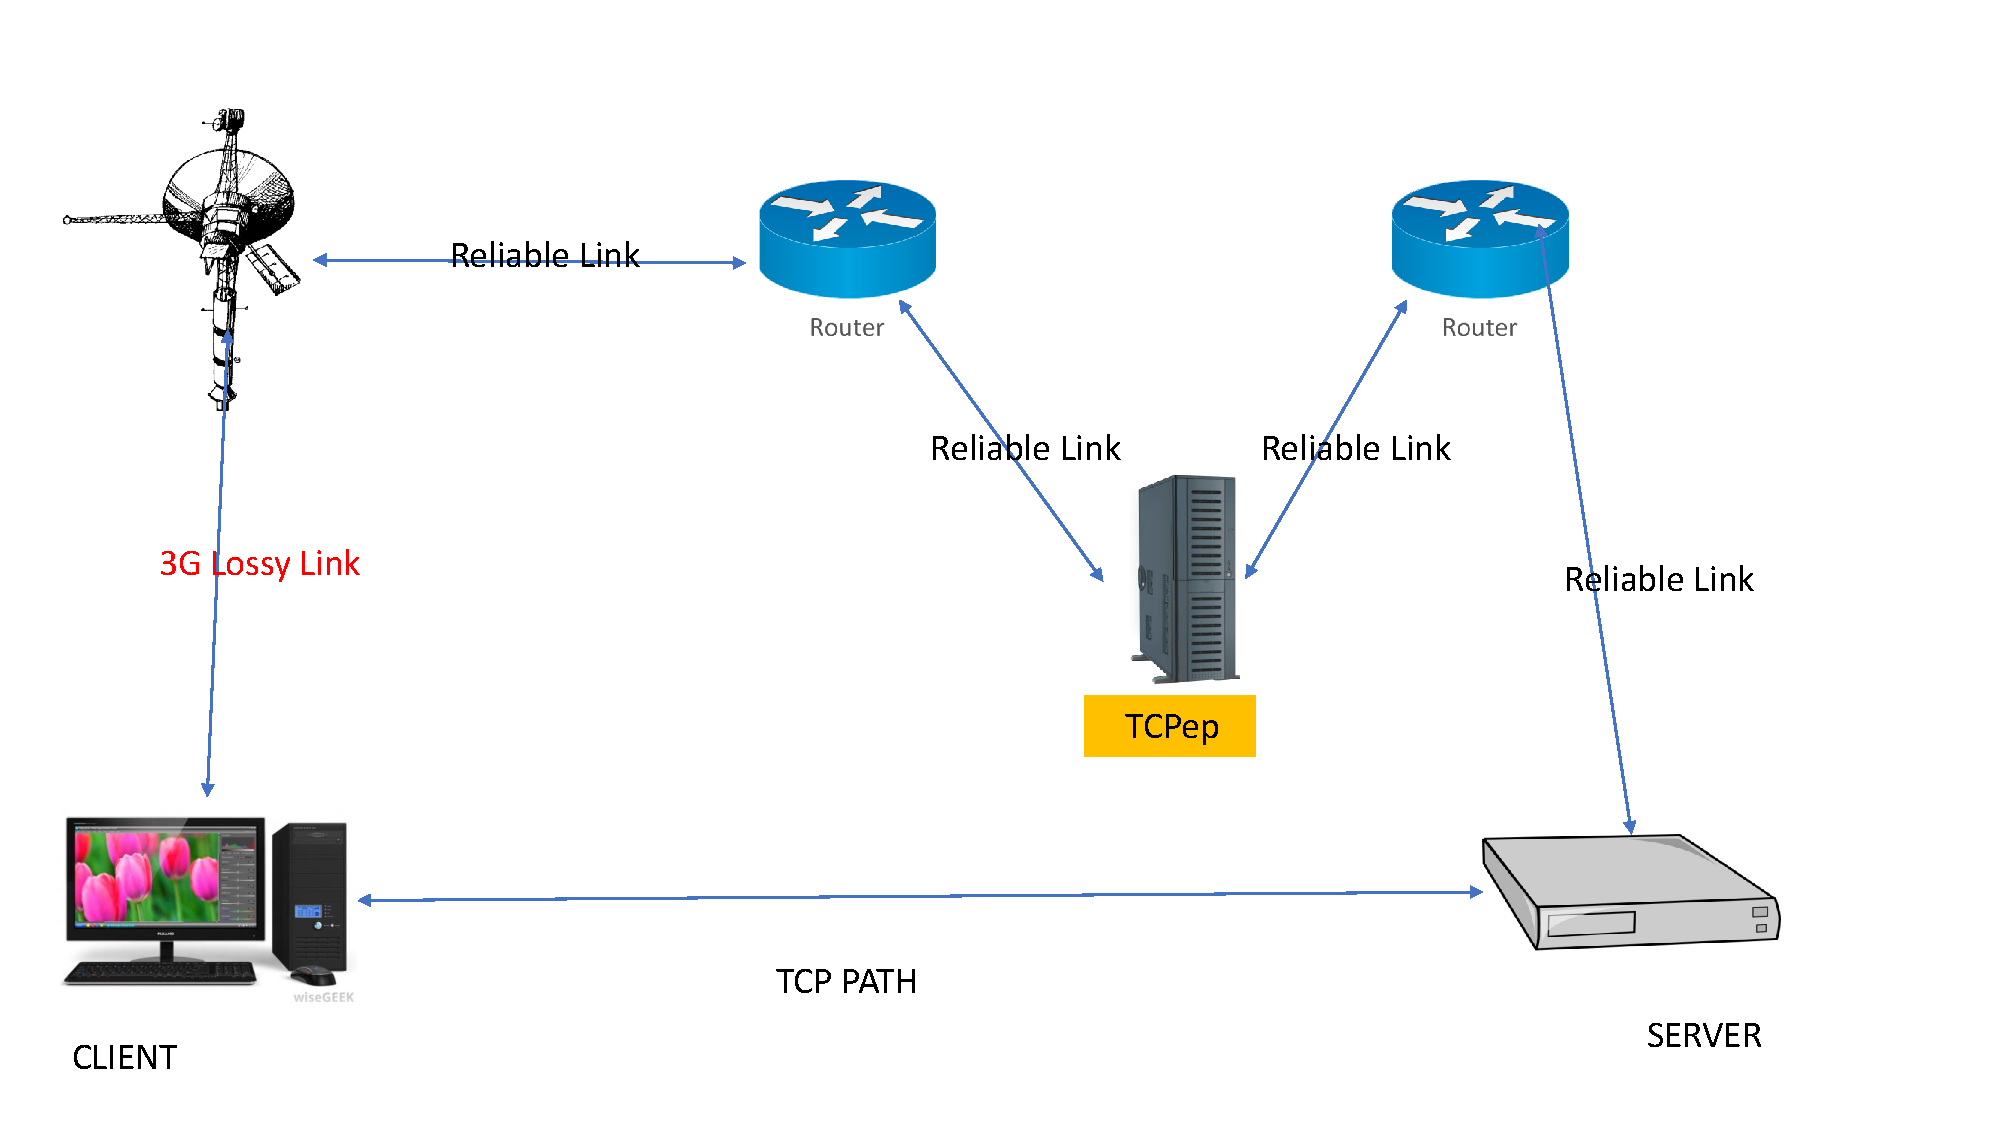
\includegraphics[width=0.9\textwidth]{TCPep.pdf}
    \caption{Typical TCPep Connection Setup}
    \label{TCPep}
\end{figure}

Therefore it was reasoned that lossy links that experience completely random losses, as has been the case in wireless links, will experience link degradation because the TCP connections are "spending excessive time in congestion avoidance and/or slow start procedures triggered by packet losses due to transmission errors" ~\cite{6}, because such losses are mistakenly treated as the result of congestion. Slow Start, for example, would assume there is congestion on the network and decrease its cwnd unnecessarily leading to undesirable results. TCPep was specifically developed to counter this type of link degradation ~\cite{33}.

TCPep makes use of network coding and an advanced algorithm to counter these effects. This thesis will not go deeply into those details as it is designed mostly for random losses on lossy links rather than queue drop losses caused by long RTT times in satellites. If the reader may wish to research more on network coding for TCPep, see section 2.2.5. 

\subsubsection*{TCPep connection type}
With TCPep, the PEP categorisation is not as important as the motivation behind its creation. We have already given an in-depth description of PEP categorisations earlier, and this one does not differ so much from the PEPsal example, so will keep it very brief here. (Differences with commercial PEPs are worth mentioning, however, so slightly more detail will be given on the categorisations when discussing commercial PEPs). 

\subsubsection*{TCPep distribution type}
TCPep is an open source integrated PEP ~\cite{33}. 

\subsubsection*{TCPep layering type}
TCPep is a transport layer PEP ~\cite{33}.

\subsubsection*{TCP splitting}
TCPep is a TCP splitting PEP ~\cite{33}.

\subsubsection*{TCPep symmetry type}
TCPep is an asymmetric PEP ~\cite{33}.

\subsubsection*{TCPep transparency type}
TCPep is transparent to the TCP hosts and end users in the network layer ~\cite{33}. 

\subsection{Commercial PEPS} 
Commercial PEPS are usually classified as proprietary "black boxes" ~\cite{6}. In other words, the network degradation protocols/solutions they use in their PEPs are not divulged to anyone in academia or the general public. PEP vendors will not necessarily be keen to submit to an academic study as they could be wary of getting unflattering results that could adversely affect sales. These vendors are also in competition with other commercial entities so it is understandable that they would want to be secretive about their methods. Any material with information on these PEPs is usually comes in the form of sales material. Naturally, one cannot expect this information to be objective and it is likely that the information presented would be overly optimistic about the effectiveness of its product ~\cite{6}. There is also the financial barrier of having to buy a commercial PEP in order to to perform an analysis on it in a study such as this. These reasons make it difficult to study commercial PEPs objectively, therefore they are beyond the scope of this thesis, but we will examine one commercial PEP (FastSAT) for the sake of an analytical comparison ~\cite{34}.\\

Unlike the previous two PEPS, commercial PEPS are costly and usually distributed (not integrated). The architecture for a typical commercial PEP can have several black box PEPs along the degraded link with modifications made to the endpoints to accommodate and maintain/enhance the throughput and reliability of the degraded network link. As Figure \ref{FastSat} shows, we have a commercial PEP called FastSAT that shows two PEPs located on both ends of the satellite link ~\cite{6}~\cite{34}. \\

FastSAT advertises "A satellite link specific, highly optimised, Flight Protocol (FP) is used for the satellite link instead of the standard TCP protocol. Alternatively, an interoperable TP protocol can also be automatically selected" ~\cite{34}. \\

In other words, it uses its own proprietary protocol tailored specifically for Satellite links and similarly degraded links affected by long RTT times. It does not, however, say exactly how its FP protocol works, what algorithm it uses etc., anywhere in its advertisement pages. The system is offered as a "black box" ~\cite{34}. \\

\subsubsection*{FastSAT distribution type}
FastSAT is a distribution type PEP, like most commercial PEPs.  As Figure 3.6 shows, FastSAT PEPs are distributed on both sides of the degraded link ~\cite{34}.

\subsubsection*{FastSAT layering type}
This FastSAT PEP operates at the Transport Layer. It replaces the TCP protocol with its own proprietary protocol FP which is designed specifically for throughput optimisation in satellite link environments. Exactly how its protocol achieves this is a trade secret, as is commonly the case with commercial PEPs ~\cite{34}. 

\subsubsection*{FASTSAT TCP splitting/protocol alteration}
FastSAT uses the TCP splitting method as does PEPsal, but it also modifies the protocol so it can be categorised under both headings. It acts as an unseen intermediary middleman between two endpoints (TCP Splitting) and deploys its own proprietary protocol FP ~\cite{34}.

\subsubsection*{FastSAT transparency type}
FastSat falls under the transparency category. As mentioned earlier, there are four degrees of transparency. Its degree of transparency is "transport layer transparency" because it is transparent with respect to the transport endpoints whom the middleware proxies are sending spoofed communications to ~\cite{34}. \\

\begin{figure}[ht!]
    \centering
    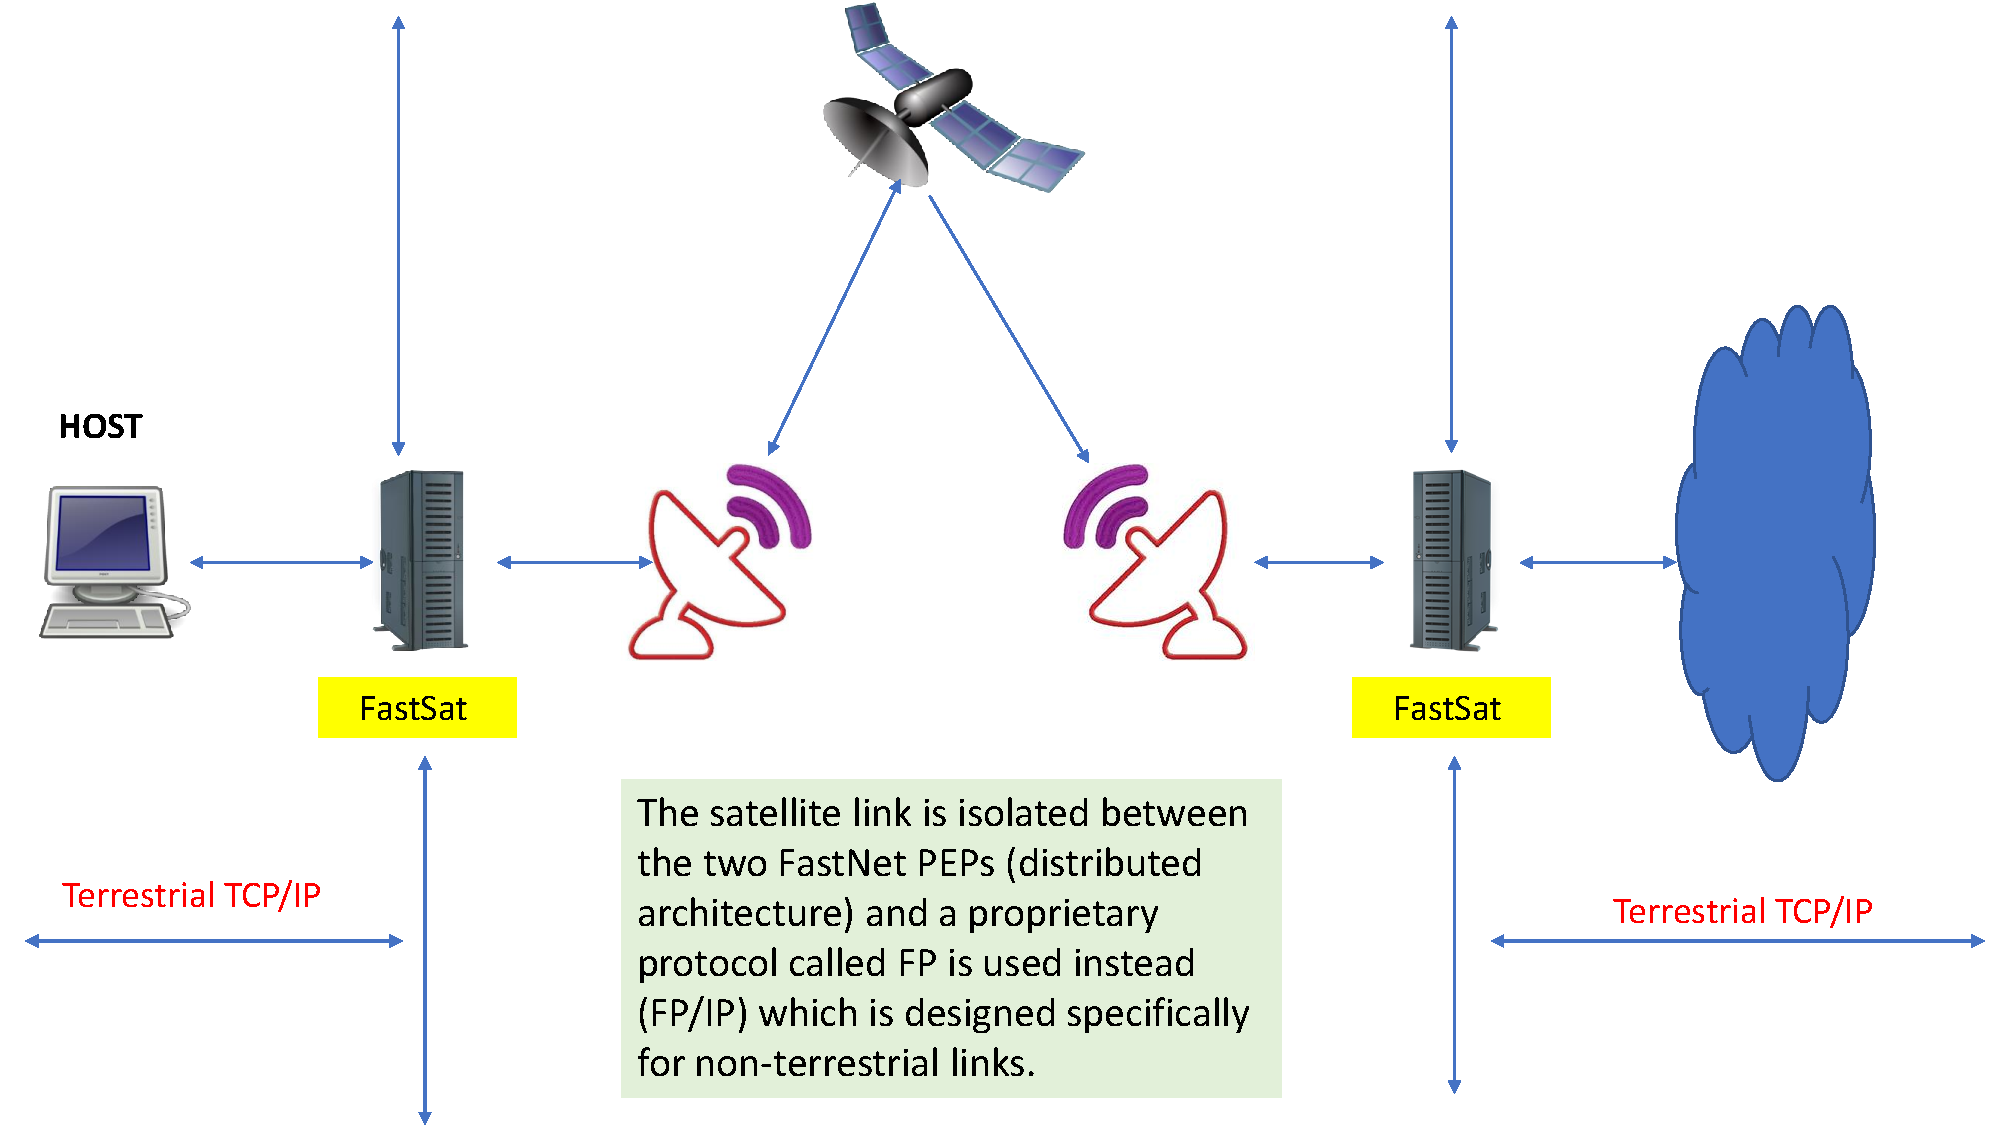
\includegraphics[width=0.9\textwidth]{FP.pdf}
    \caption{Proprietary FP Protocol}
    \label{FastSat}
\end{figure}

\subsubsection*{Summary}
In summary, this chapter has covered three different kinds of PEPs that were based on differing motivations and employing different strategies for resolving link degradations. The PEPs were also categorised according to standard RFC PEP classifications to highlight the variety of PEP functionalities and features available, but without getting bogged down in too much technical detail.  In the next chapter, details of our proposed solution takes the reader through the methods used for creating our PEP.



